\documentclass{article}
\usepackage{indentfirst}
\usepackage[utf8]{inputenc}
\usepackage[T1]{fontenc}
\usepackage[brazilian]{babel}
\usepackage{lmodern}
\usepackage{graphicx}
\usepackage{float}
\usepackage[]{subfigure}
\usepackage{afterpage}
\usepackage{amsmath}
\usepackage{textcomp,gensymb}
\usepackage{nameref}
\usepackage{accents}
\usepackage{listings}
\usepackage{color,soul}
\usepackage[margin=1in]{geometry}
\usepackage{steinmetz}

\PassOptionsToPackage{hyphens}{url}\usepackage{hyperref}
\hypersetup{
    breaklinks = true,
}
\urlstyle{same}
\newcommand{\ubar}[1]{\underaccent{\bar}{#1}}
\renewcommand\thesection{\arabic{section}$^a$}
\renewcommand\thesubsection{\arabic{section}.\alph{subsection}}
\definecolor{dkgreen}{rgb}{0,0.6,0}
\definecolor{gray}{rgb}{0.5,0.5,0.5}
\definecolor{mauve}{rgb}{0.58,0,0.82}
\lstset{
    frame=tb,
    language=Matlab,
    aboveskip=3mm,
    belowskip=3mm,
    showstringspaces=false,
    basicstyle={\small\ttfamily},
    numbers=none,
    numberstyle=\tiny\color{gray},
    keywordstyle=\color{blue},
    commentstyle=\color{dkgreen},
    stringstyle=\color{mauve},
    breaklines=true,
    breakatwhitespace=true,
    tabsize=4
}

\title{Trabalho}
\author{Arthur Matos}
\date{2017}

\begin{document}
% capa
\begin{titlepage}
    \begin{center}
        \centering
        
\includegraphics[width=.7\linewidth]{images/logo_unb.png}\\[0.5cm]
        {\large \textbf{Universidade de Brasília}}\\[0.2cm]
        {\large \textbf{Departamento de Engenharia Elétrica}}\\[0.2cm]
        {\large \textbf{Controle Digital}}\\[4.8cm]
        {\bf \huge {Exercício de Simulação 1}}\\[0.2cm]
        {\bf \large {}}
    \end{center}

    \vspace{5cm}
    \hspace{2cm} {\noindent \bf \large {Aluno:}}\\
    \vspace{0.8cm}
    \hspace{2.35cm} {\large Arthur de Matos Beggs --------------------------------- 12/0111098}\\[1cm]

    \begin{center}
        {\large Brasília}\\
        {\large 1$^{\ubar{\circ}}$/2019}
    \end{center}

\end{titlepage}
\clearpage
\setcounter{page}{2}
% \tableofcontents
\clearpage

% % Template de figura
% \begin{figure}[H]
%     \centering
%         \includegraphics[width=1\linewidth]{images/}
%         \caption{}\label{fig:}
% \end{figure}

% % Corpo do Relatório

{\Large \bf {
    Considere um sistema de controle a tempo discreto com realimentação
    unitária e período de amostragem $ T = 1s $ cuja função de transferência é
    dada por

    \[ G(z) = \frac{K(0.379z + 0.2642)}{(z-0.3679)(z-1)} \]
}}

\begin{figure}[H]
    \centering
        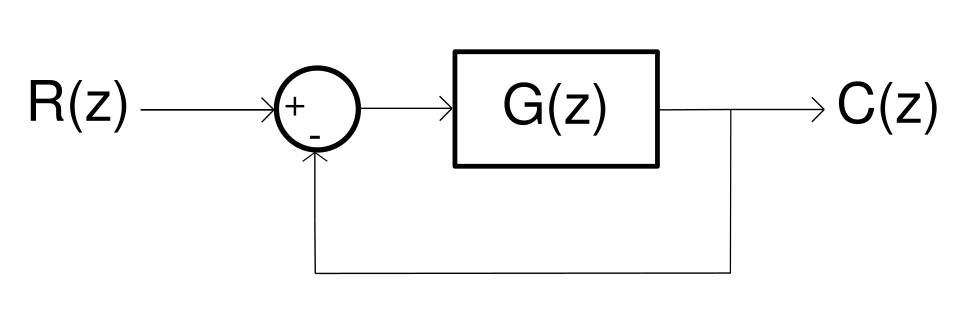
\includegraphics[width=.6\linewidth]{images/block_diagram.png}
        \caption{Diagrama de blocos do sistema}\label{fig:block}
\end{figure}

\section{Usando o critério de Jury, determine o intervalo de valores de $K$
    para o qual o sistema em malha fechada é estável
}

    \[ \frac{C(z)}{R(z)} = \frac{G(z)}{1 + G(z)} = \frac{K(0.3679z + 0.2642)}{z^2 + (0.3679K - 1.3679)z + 0.3679 + 0.2642K} \]\\

    {O polinômio característico $P(z)$ é dado por}

    \[ P(z) = z^2 + (0.3679K - 1.3679)z + 0.3679 + 0.2642K \]\\

    {Assim, seus coeficientes são}

    \[ a_0 = 1\qquad  a_1 = 0.3679K - 1.3679\qquad a_2 = 0.3679 + 0.2642K \]\\

    {Analisando os critérios de Jury, temos}

    \begin{enumerate}
        \item $ |a_2| < a_0 \implies |0.3679 + 0.2642K| < 1 $
            \[
                \begin{cases}
                    0.3679 + 0.2642K < 1  & \quad \implies k < 2.3925\\
                    -0.3679 - 0.2642K < 1 & \quad \implies k > -5.1775
                \end{cases}
            \]
        \item $ P(1)  > 0 \implies P(1)  = 0.6231K > 0 \implies K > 0 $
        \item $ P(-1) > 0 \implies P(-1) = 1 - (0.3679K - 1.3679) + 0.3679 + 0.2642 > 0 \implies K < 2.3925 $
    \end{enumerate}

    \begin{figure}[H]
        \centering
            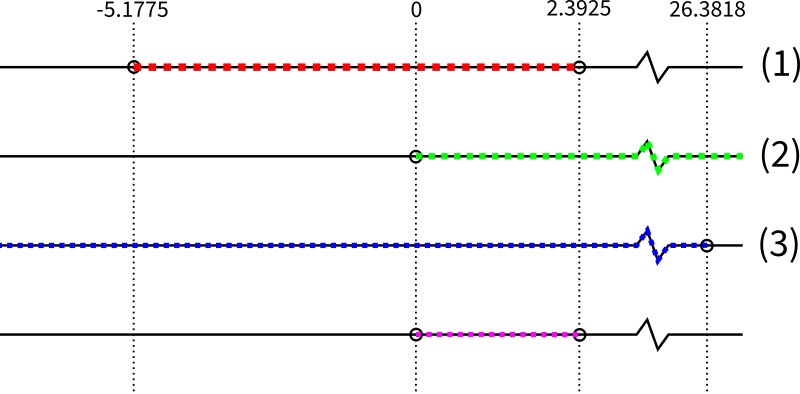
\includegraphics[width=.5\linewidth]{images/k_intervals.png}
            \caption{Intervalos de valores para K}\label{fig:intervals}
    \end{figure}

    {Assim, o sistema é estável para $ 0 < K < 2.3925 $.}

\section{Repita o item anterior usando o critério de Routh Modificado}

    {O critério de Routh-Hurwitz modificado mapeia o domínio $s$ no domínio $z$
    utilizando a transformação}

    \[ z = \frac{s + 1}{s = 1} \]

    {Aplicando a transformação em $P(z)$, temos}

    \[ P(z) = z^2 + (0.3679K - 1.3679)z + 0.3679 + 0.2642K \]
    \[ P(s) = {\left(\frac{s + 1}{s - 1}\right)}^2 + (0.3679K - 1.3679)\left(\frac{s + 1}{s - 1}\right) + 0.3679 + 0.2642K \]
    \[ P(s) = (0.6321K)s^2 + (1.2642 - 0.5284K)s + (2.7358 - 0.1037K) \]\\

    {Montando a tabela de Routh-Hurwitz,}

    \begin{table}[H]
        \centering
        \begin{tabular}{ c | l }
            $s^2$ & $0.6321K$ \\
            $s^1$ & $(1.2642 - 0.5284K)$ \\
            $s^0$ & $(2.7358 - 0.1037K)$ \\
        \end{tabular}
    \end{table}

    {Para $s > 0$,}

    \begin{itemize}
        \item $ 0.6321K > 0 \quad \implies K > 0 $
        \item $(1.2642 - 0.5284K) > 0 \quad \implies K < \frac{1.2642}{0.5248} \quad \implies K < 2.3925 $
        \item $(2.7358 - 0.1037K) > 0 \quad \implies K < \frac{2.7358}{0.1037} \quad \implies K < 26.3818 $
    \end{itemize}

    {O intervalo $ 0 < K < 2.3925 $ satisfaz as condições quando $s > 0$.}\\

    {Para $s < 0$,}

    \begin{itemize}
        \item $ 0.6321K < 0 \quad \implies K < 0 $
        \item $(1.2642 - 0.5284K) < 0 \quad \implies K > \frac{1.2642}{0.5248} \quad \implies K > 2.3925 $
        \item $(2.7358 - 0.1037K) < 0 \quad \implies K > \frac{2.7358}{0.1037} \quad \implies K > 26.3818 $
    \end{itemize}

    {Não há intervalos de valores de $K$ que satisfaçam as condições quando $s < 0$.}\\

    {Assim, o sistema é estável para $ 0 < K < 2.3925 $.}


\section{Determine o valor de K para o qual o sistema a malha fechada apresenta
    resposta ao degrau oscilatória com amplitude constante. Determine também a
    frequência de oscilação correspondente
}

    {De acordo com os intervalos para K encontrados nas questões anteriores,
    tomando os valores nos limites de K, temos que:}

    \[ \text{Para } K = 0, \quad C(z) = 0 \; \forall \; R(z) \]

    \[ \text{Para } K = 2.3925, \quad P(z) = z^2 - 0.4877z + 1 \]
    \[    z = 0.2439 \pm j 0.9698 \]
    \[    |z| = \sqrt{0.2439^2 + 0.9698^2} = 1 \]

    {Assim, para $ K = 2.3925 $, o sistema possui pólos no Círculo de Raio
    Unitário, e oscila com amplitude constante. Para determinar a frequência de
    oscilação quando $ K = 2.3925 $,}

    \[ z = e^{s T} = e^{j \omega T} = 1 \phase{\omega_n T} \]

    \[ \phase{z} = \arctan \frac{0.9698}{0.2439} = 1.3244 rad = \omega_n T \]

    {Como $ T = 1s $, $ \omega_n = 1.3244 rad/s $.}


\section{Simule o sistema no Simulink usando o bloco de função de transferência
    discreta para referência degrau unitário. Escolha valores de K de modo que
    a resposta do sistema seja estável, instável e marginalmente estável.
    Verifique se a frequência de oscilação da resposta marginalmente estável é
    igual a calculada no item anterior. Apresente o diagrama de simulação e os
    gráficos das respostas obtidas.
}

    {Para o sistema com resposta estável, foi escolhido $K = 1$.}

\begin{figure}[H]
    \centering
        \includegraphics[width=.8\linewidth]{images/Simulink_diagram_stable.jpg}
        \caption{Diagrama do sistema com resposta estável}\label{fig:diagram_stable}
\end{figure}

\begin{figure}[H]
    \centering
        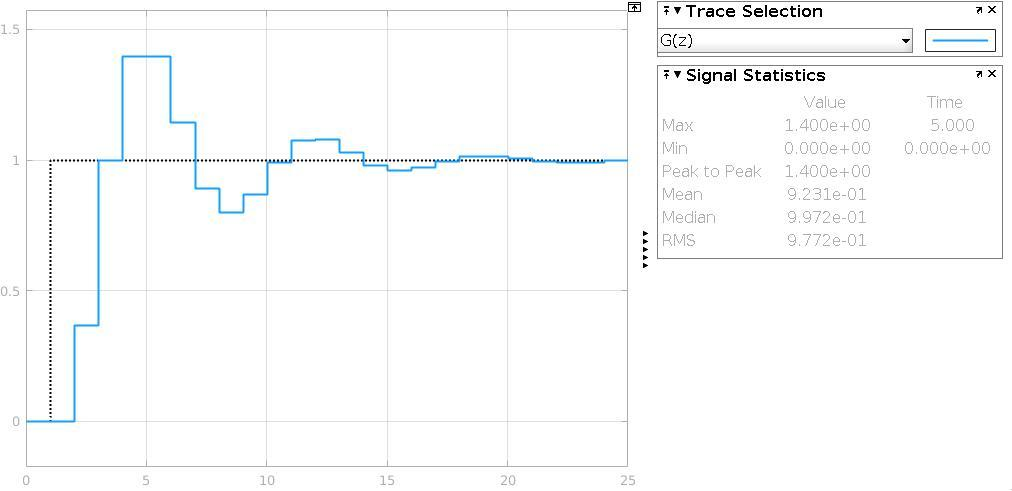
\includegraphics[width=.8\linewidth]{images/simulink_scope_stable.jpg}
        \caption{Gráfico da resposta estável}\label{fig:scope_stable}
\end{figure}

    {Para o sistema com resposta instável, foi escolhido $K = 3$.}

\begin{figure}[H]
    \centering
        \includegraphics[width=.8\linewidth]{images/Simulink_diagram_unstable.jpg}
        \caption{Diagrama do sistema com resposta instável}\label{fig:diagram_unstable}
\end{figure}

\begin{figure}[H]
    \centering
        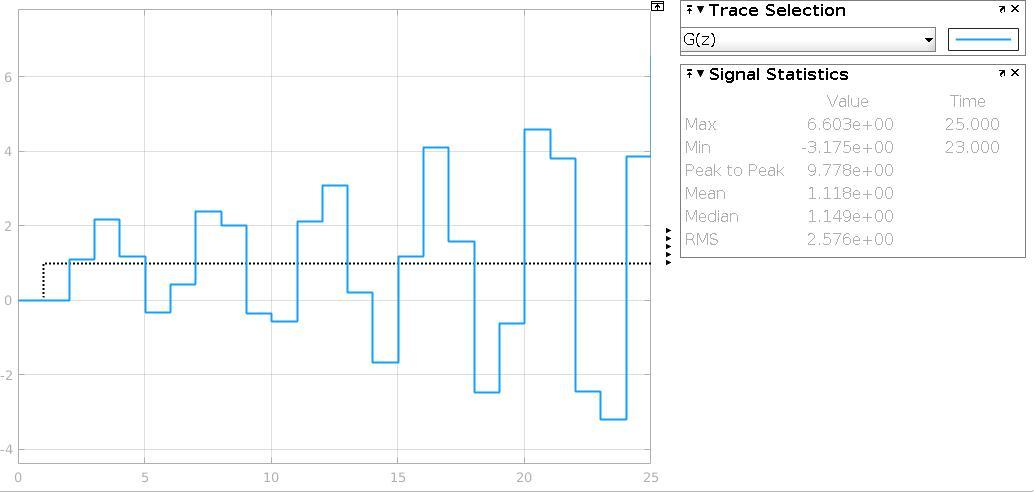
\includegraphics[width=.8\linewidth]{images/simulink_scope_unstable.jpg}
        \caption{Gráfico da resposta instável}\label{fig:scope_unstable}
\end{figure}

    \clearpage
    {Para o sistema com resposta marginalmente estável, foi escolhido $K = 2.3925$.}

\begin{figure}[H]
    \centering
        \includegraphics[width=.8\linewidth]{images/Simulink_diagram_marginally_stable.jpg}
        \caption{Diagrama do sistema com resposta marginalmente estável}\label{fig:diagram_marginally_stable}
\end{figure}

\begin{figure}[H]
    \centering
        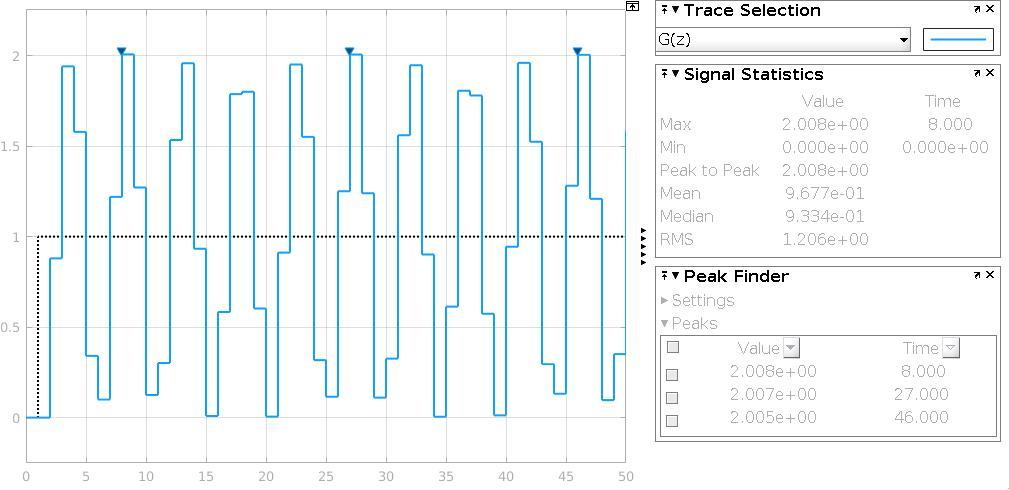
\includegraphics[width=.8\linewidth]{images/simulink_scope_marginally_stable.jpg}
        \caption{Gráfico da resposta marginalmente estável}\label{fig:scope_marginally_stable}
\end{figure}

    {Os picos ocorrem nos instantes $8s$, $27s$ e $46s$. Como o sinal oscila
    quatro vezes entre um pico e o seguinte, o período de oscilação é dado por}

    \[ 27 - 8 = 46 - 27 = 19s \]

    \[ \frac{19s}{4} = T = 4.75s \]

    \[ \omega_n = \frac{2 \pi}{T} \approx 1.3228 rad/s \approx 1.3244 rad/s \]

    {O valor da frequência de oscilação encontrado na simulação é aproxiamdamente
    igual ao valor calculado.}


\end{document}

